\chapter{Related Work}\label{cha:Related}

\section{MOOCs}

\subsection{Overview}
MOOCs refers to massive online open courses, which is a online course platform people can access through internet connection regardless of the limit of space and time.
MOOCs is normally free, credit-less and is designed for massive people to enroll and learn.
Base on different theories, there are two kinds of MOOCs, cMOOCs and xMOOCs, which will mentioned in following section.

\subsection{cMOOCs v.s. xMOOCs}
Since ``The year of MOOCs'' \cite{pappano2012}, MOOCs have become increasingly robust and diverse in last few year.
There are many websites provide MOOCs for different group in various way.
Based on different learning theory, we classify MOOCs into cMOOCs and xMOOCs.
cMOOCs are base on the learning theory of Connectivism, this kind of MOOCs focus on network between individuals in course.
students may use any digitle platform such as Facebook, Google+, blog to make connections with other learners to create and construct knowledge.
The participants in cMOOCs act as teacher and learner at the same time as they share knoledge with each other.
Instead of being structured as an open online community of learners, xMOOCs are much more like traditional classroom environment.
xMOOCs are centered around class instroctor, instroctor usually will provide series of lecture video, where learners mainly get knowledges.
Besides, exercises, quizes, assignments are also used during the course.
Most of the popular MOOC websites in recent year are belong to xMOOCs such as Coursera, edX, Udacity, etc.

\subsection{Coursera}

\begin{figure}[H]
    \centering
    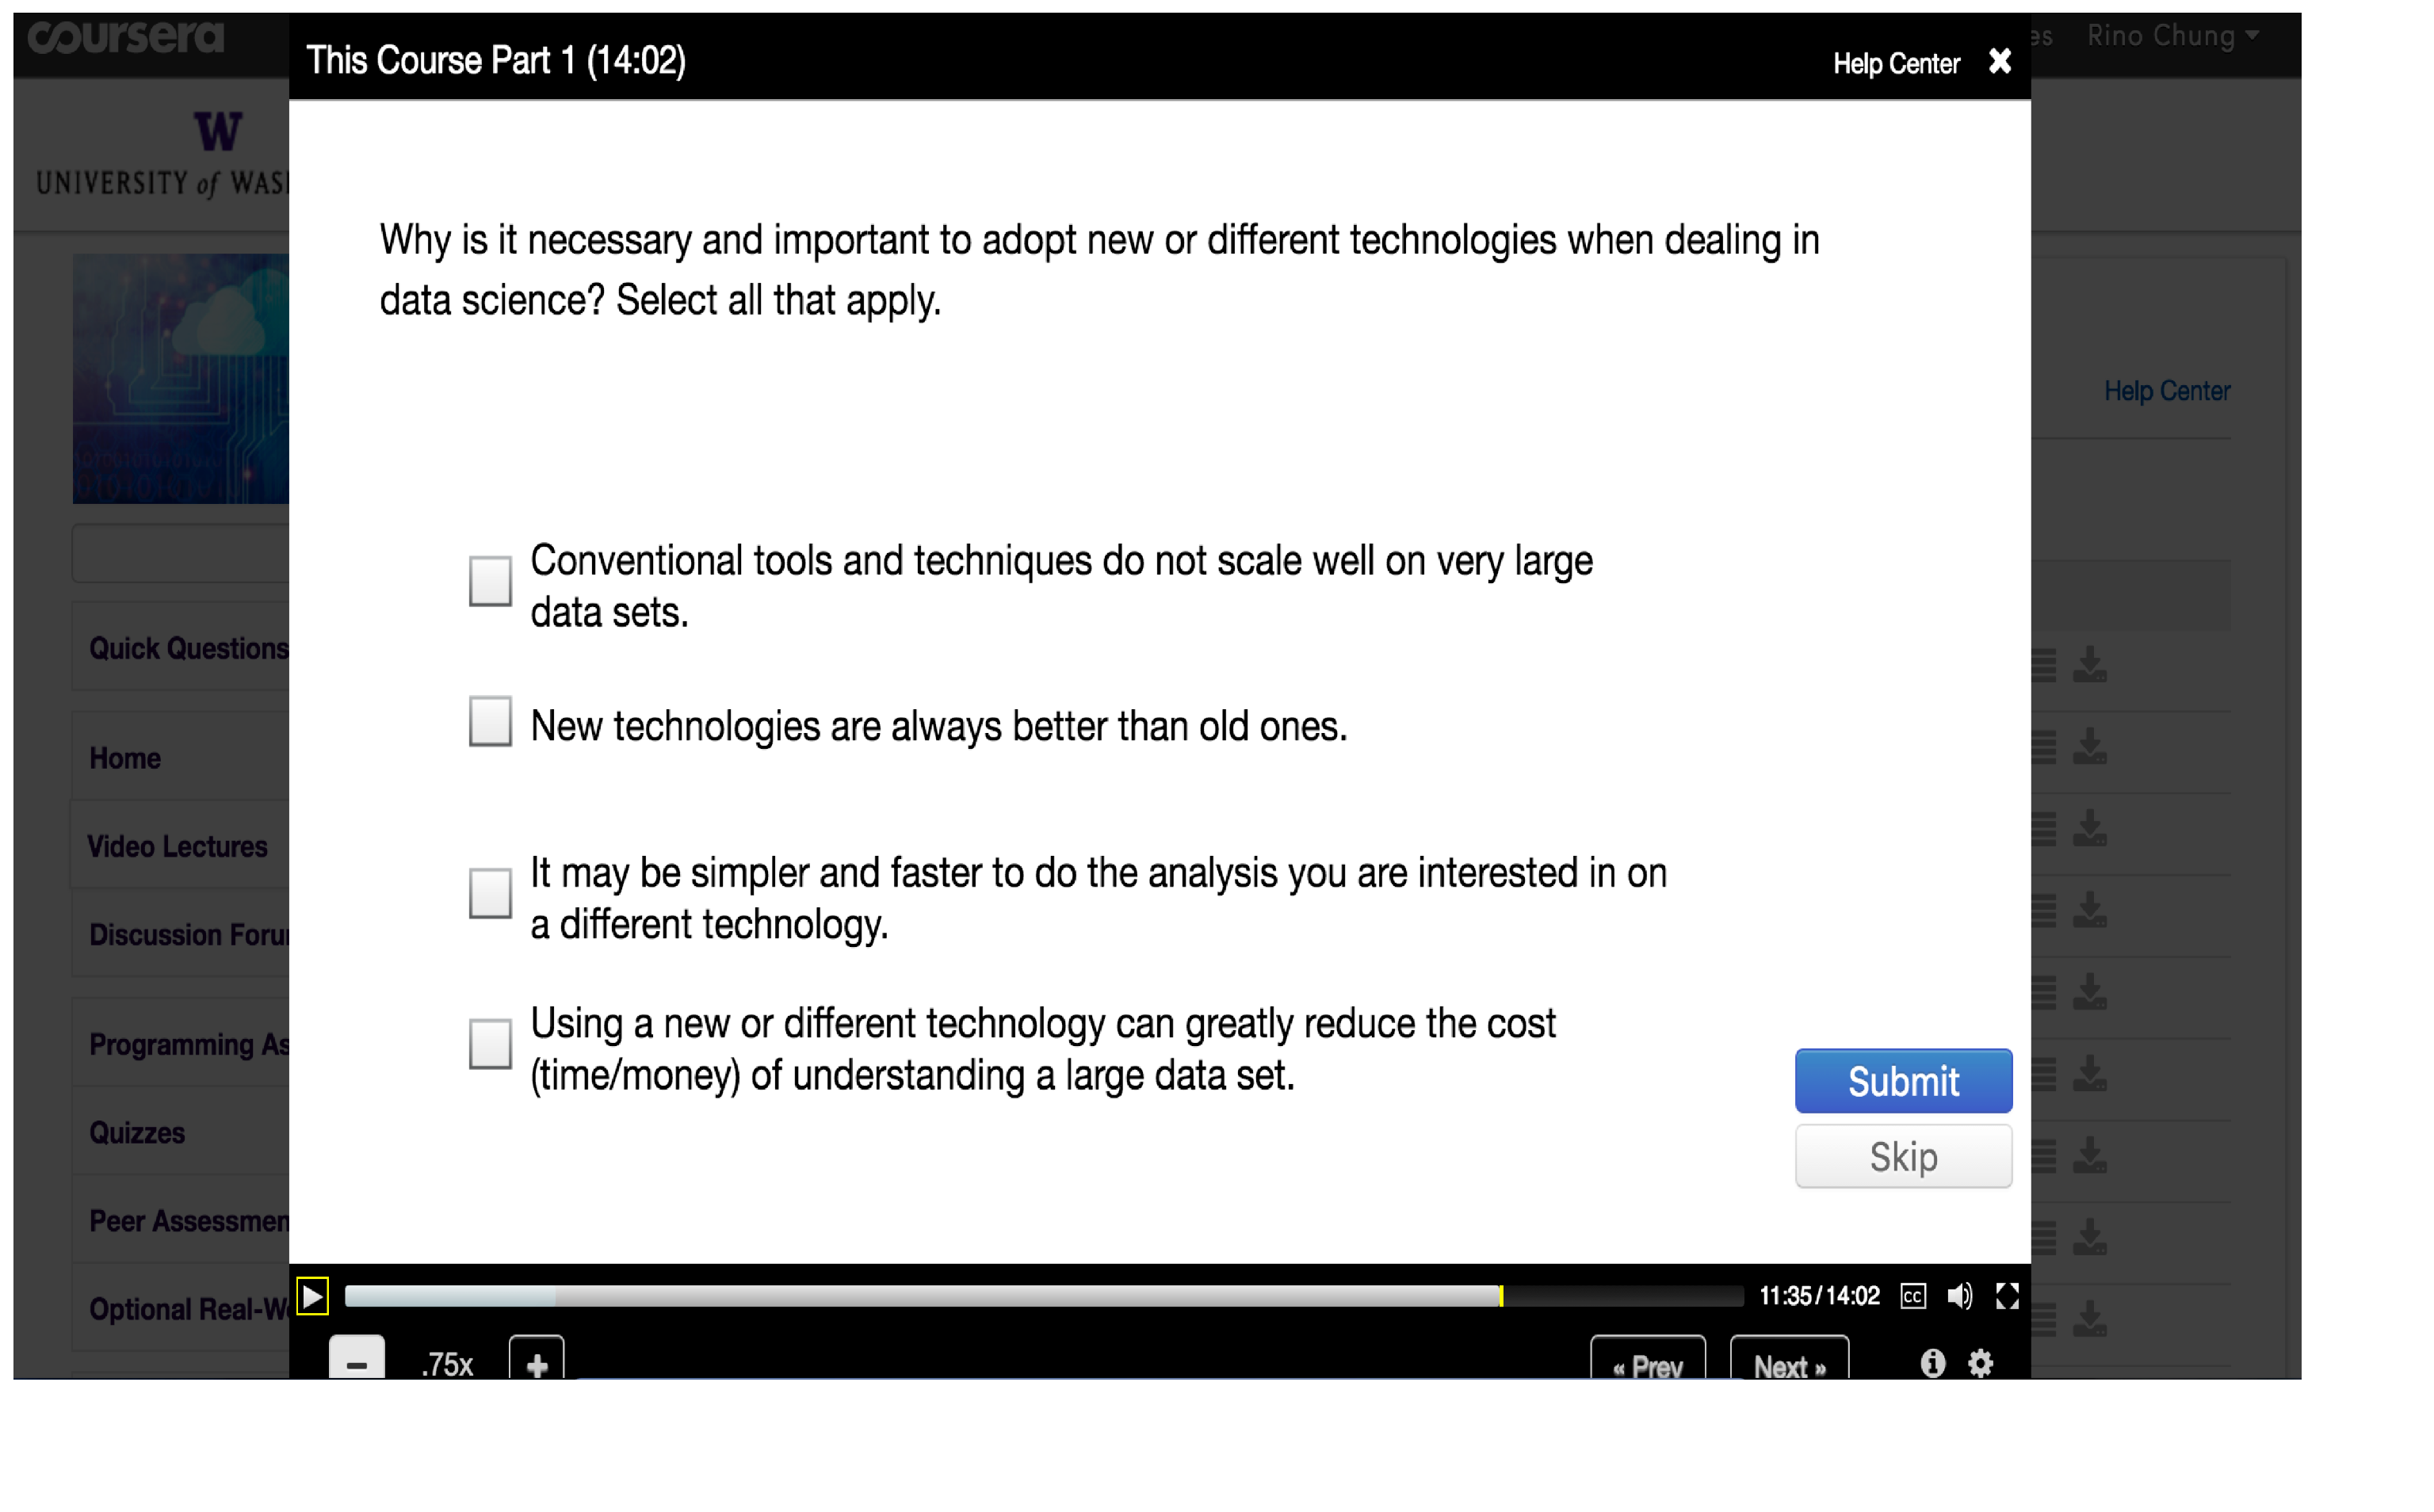
\includegraphics[width = 0.8\textwidth]{fig/coursera_pop.eps}
    \caption{Coursera pop-up question in lecture video}
    \label{fig:coursera_pop}
\end{figure}

Coursera \cite{coursera} started in 2012 founded by Stanford University. It provides courses from renowned universitise like Stanford University,  Princeton University, University of Michigan, etc.
Taking course on Course is free, learners can enroll courses that interest them at will.
Applying for hard copy certification of course, however, will charge for some money.
As a xMOOC platform, lecture videos are the major teaching material of courses with transcripts in many different language, usually after every one of two lecture video there will be a execise for user to check if the had understand previous content of videos; moreover forum, quiz, assignments and other traditional xMOOC functions are also provide on Coursera.
To make sure learners focusing on the lecture video, there is a pop-up question about current video in every lecturevideo see Figure \ref{fig:coursera_pop}.
The question will let you submit three times, and if all the answers are wrong in three submission system will tell you the answer but learners can chose to continue the video without answering the question.
Coursera also has iOS, Android, and Kindle Fire apps.

\subsection{edX}
edX \cite{edx} is also a xMOOC platform, which founded by Harard University and MIT at 2012 offering high-quality courses from universities and intuitions to learners.
As a xMOOC too, edX and Coursera are pretty alike. Free for taking courses, center on lecture videos whit the supports like forum, exam, and other features most MOOC platform has.
Similar to Coursera, edX has a certificate system, which you can apply for hard copy proof when you pass the course; it will charge you certificate fee, however, the price is slightly lower than Coursera.
Besides the majority of courses are taught in english, edX also provides some foreign language courses.
\begin{figure}[H]
    \centering
    \includegraphics[width = 0.8\textwidth]{fig/edx.eps}
    \caption{edX transcript redirect function: redirect video to specific section by transcript content}
    \label{fig:edx}
\end{figure}
edX has transcript redirect function on the right of the player see Figure \ref{fig:edx}.
This function is helpful for learners to know what is the video talks about before go through the whole video or help them easier to target the segment they what to replay again.

\subsection{Open edX}
Open edX is a free and open source course management system that was originally developed by edX.
Among Open edX, there are many useful tool or model for constructing a course already be done, see Table \ref{table:edxfeature}.
With the help of Open edX, people around the word can build and host their own MOOC, take xuetangx \cite{xuetangx} for example, a famouse MOOC website in China for chinese speaking learners that built based on Open edX.

\begin{table}[H]
\centering
\caption{Open edX features}
\label{table:edxfeature}
\begin{tabular}{|c|p{12cm}|}
\hline
Feature           & \multicolumn{1}{c|}{Description}                                                                                                                                                                                                                                                                                                                                                                                                                                                                                    \\ \hline
Open edX Studio   & Studio is the Open edX tool that used to build courses, which provided with a GUI interface make users easily edit courses through a browser. You use Studio to create the course structure and then edit course content, including problems, lecture videos, and other resources for learners. You also use Studio to manage the course schedule and the course team(instructors, tutors), set grading policies, publish each part of your course, and more.                                                       \\ \hline
LMS               & LMS in the Open edX is a tool that learners use to access course resources and to check their learning progress in the course. The Open edX LMS can also offer a discussion forum and a wiki that both learners and course team members can contribute to.                                                                                                                                                                                                                                                          \\ \hline
XBlock            & XBlock is the component architecture for the elements of an Open edX course. Platform developers can adjust course components to meet instructors' need. For instance, you can build XBlocks to represent course contents such as problems, text string, or HTML content to implement interactive learning laboratories. The primary advantage of XBlocks is that they are deployable in any edX Platform or other XBlock application, which make the code you write can be used by any course team and vice versa. \\ \hline
Open edX Insights & edX Indights is a course analytics system in Open edX, course team can use collected data to monitor learners' activities, learning patterns, reveal problems might confuse learners, or do researches base on these data to refine courses.                                                                                                                                                                                                                                                                        \\ \hline
\end{tabular}
\end{table}

\subsection{Data-Driven Analysis}
Since MOOCs are becoming increasingly popular, thousands of lecture video clickstream data are produced.
Many studies do research on applying clickstream data to observe user learning behavior and what's more, the meaning of user learning behavior \cite{linan2015}.
The information provided by user clickstream data can help not only instructor to improve but also to optimize the learning experience of lecture video watcher.
Paper \cite{Conglei2015} develops a analytic system is proposed to help analyzing user behavior by using video clickstream data (see Figure \ref{fig:vismooc}).

\begin{figure}[H]
    \centering
    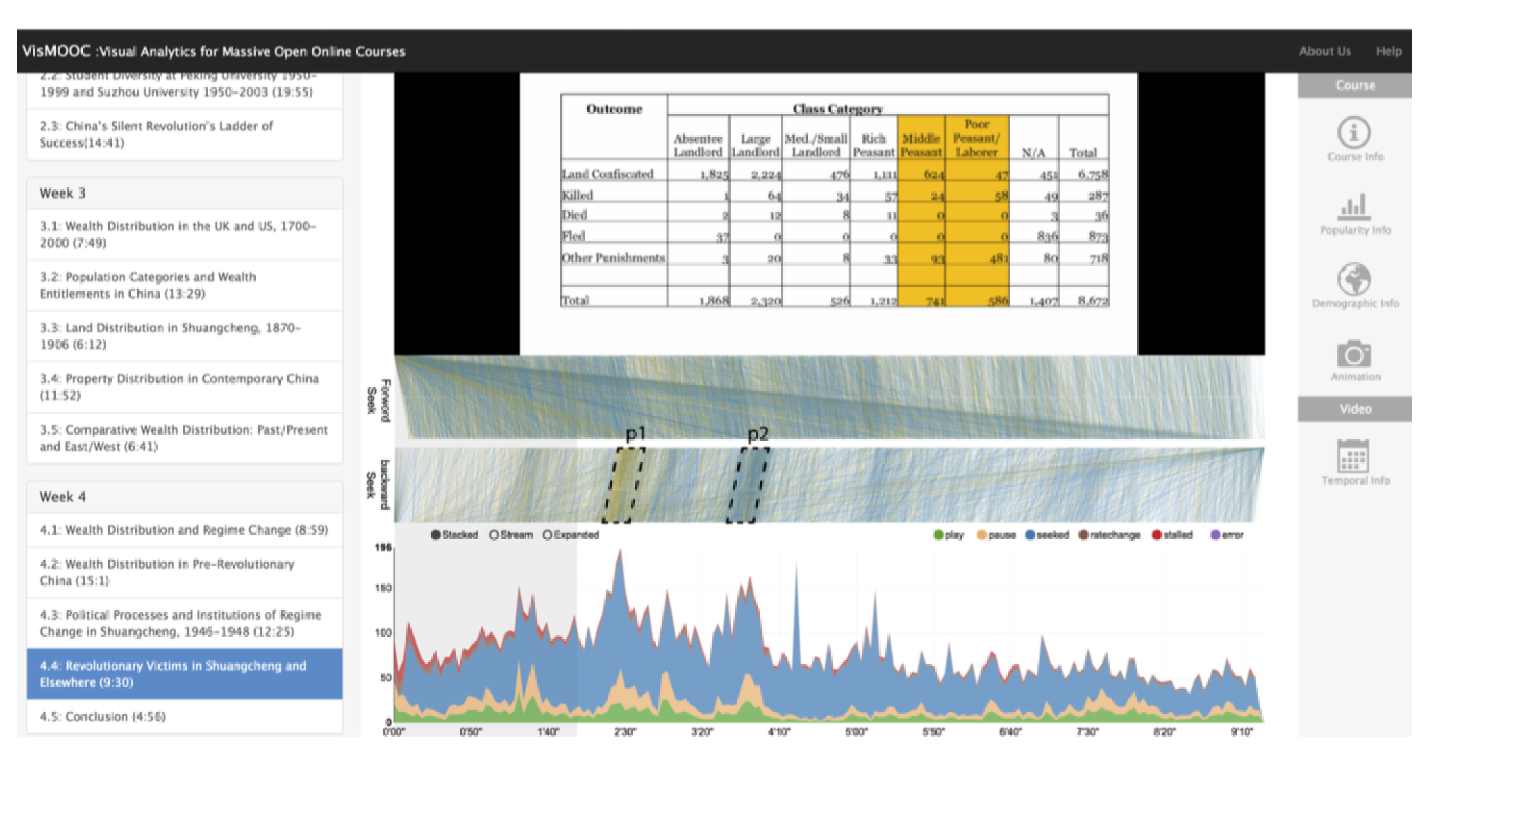
\includegraphics[width = 0.8\textwidth]{fig/vismooc.eps}
    \caption{Screenshot of visMooc}
    \label{fig:vismooc}
\end{figure}

Seek graphs analysis in visMOOC is a feature to understand leaners proactive information seeking behavior on watching videos.
From the seek graph we can observe some video segments of interest with dense seek lines \ref{fig:vismoocseek}.
In this thesis, we use the similar concept to find the hot segment.

\begin{figure}[H]
    \centering
    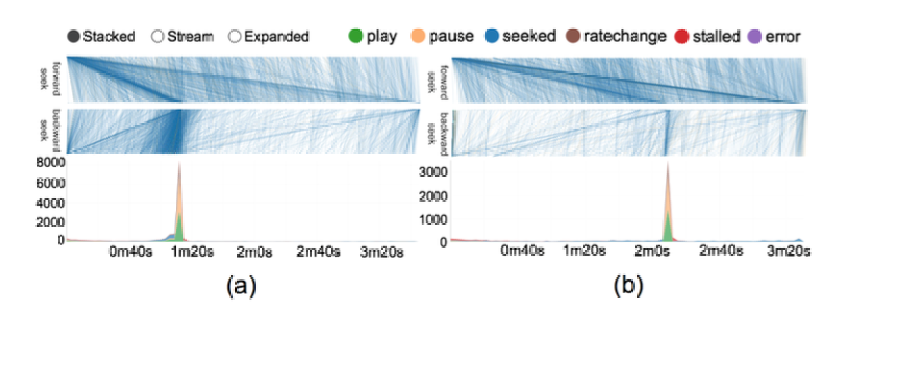
\includegraphics[width = 0.8\textwidth]{fig/vismoocseek.eps}
    \caption{visMooc Seek Graph Analysis}
    \label{fig:vismoocseek}
\end{figure}
